\section{Results – Strategy S3: Multi-LLM Consensus (Full)}
\label{sec:eval-s3}

The \textbf{S3: Multi-LLM Consensus (Full)} strategy runs multiple LLMs on the full document and aggregates their outputs with a verification/consensus step. We evaluate three variants: \textbf{S3.0} without few-shot examples on the original MUC-4 dataset, \textbf{S3.1} with few-shot examples on the original dataset, and \textbf{S3.2} with few-shot examples on a speech-style variant of MUC-4.

\begin{figure}[H]
\centering
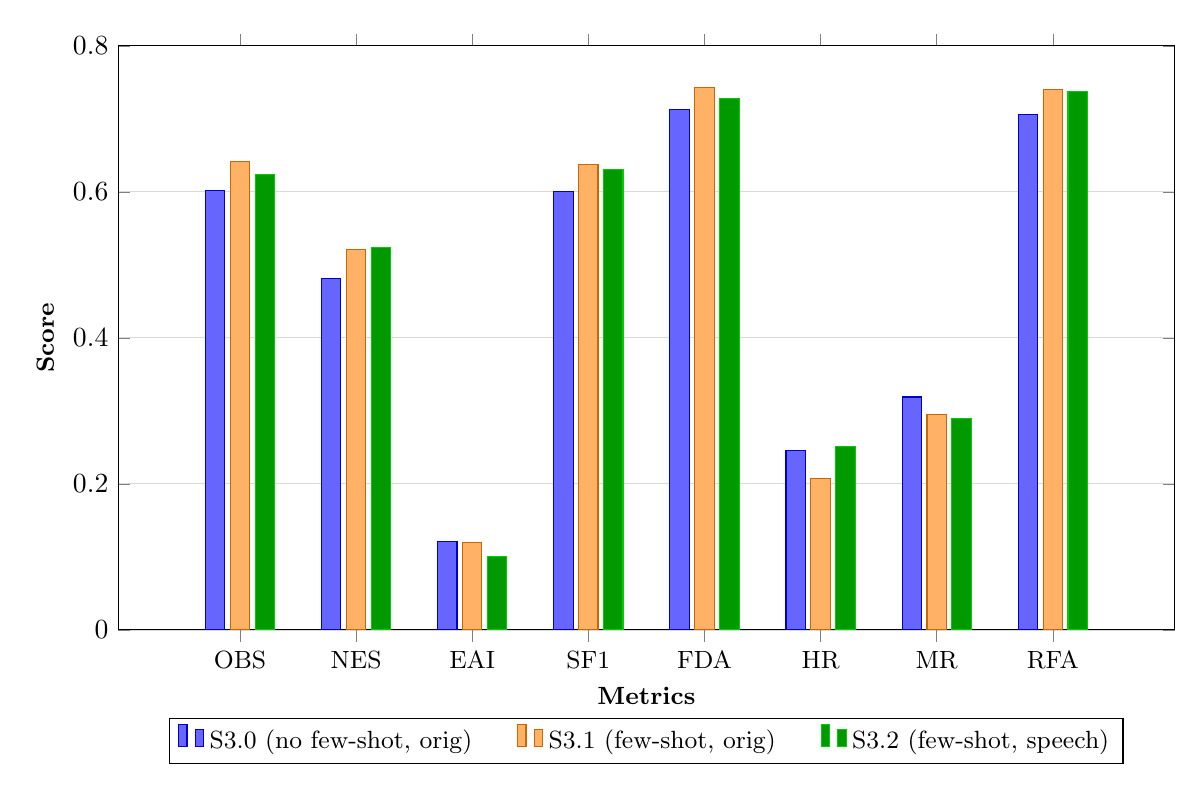
\begin{tikzpicture}
  \begin{axis}[
    width=15cm,
    height=9cm,
    ybar,
    bar width=7pt,
    ylabel={Score},
    ylabel style={font=\small\bfseries},
    xlabel={Metrics},
    xlabel style={font=\small\bfseries},
    symbolic x coords={OBS, NES, EAI, SF1, FDA, HR, MR, RFA},
    xtick=data,
    xticklabel style={font=\small},
    ymin=0,
    ymax=0.8,
    ytick={0, 0.2, 0.4, 0.6, 0.8},
    ymajorgrids=true,
    grid style={line width=0.3pt, draw=gray!30},
    legend style={
      at={(0.5,-0.15)},
      anchor=north,
      legend columns=3,
      font=\small,
      /tikz/every even column/.append style={column sep=0.5cm}
    },
    enlarge x limits=0.15,
  ]
  
  % S3.0 (no few-shot, orig) - Blue
  \addplot[fill=blue!60, draw=blue!80!black] coordinates {
    (OBS, 0.602)
    (NES, 0.481)
    (EAI, 0.121)
    (SF1, 0.601)
    (FDA, 0.713)
    (HR, 0.246)
    (MR, 0.319)
    (RFA, 0.706)
  };
  \addlegendentry{S3.0 (no few-shot, orig)}
  
  % S3.1 (few-shot, orig) - Orange
  \addplot[fill=orange!60, draw=orange!80!black] coordinates {
    (OBS, 0.641)
    (NES, 0.521)
    (EAI, 0.120)
    (SF1, 0.638)
    (FDA, 0.743)
    (HR, 0.208)
    (MR, 0.295)
    (RFA, 0.740)
  };
  \addlegendentry{S3.1 (few-shot, orig)}
  
  % S3.2 (few-shot, speech) - Green
  \addplot[fill=green!60!black, draw=green!80!black] coordinates {
    (OBS, 0.624)
    (NES, 0.524)
    (EAI, 0.100)
    (SF1, 0.630)
    (FDA, 0.728)
    (HR, 0.251)
    (MR, 0.289)
    (RFA, 0.738)
  };
  \addlegendentry{S3.2 (few-shot, speech)}
  
  \end{axis}
\end{tikzpicture}
\caption{Headline metrics for S3 variants on MUC-4 ($N{=}100$).}
\label{fig:s3-variants-bar}
\end{figure}

Figure~\ref{fig:s3-variants-bar} shows that full-document consensus with few-shot prompting yields consistently strong performance. Moving from S3.0 to S3.1 improves OBS (from $0.602$ to $0.641$) and SF1 (from $0.601$ to $0.638$), while FDA increases from $0.713$ to $0.743$ and HR drops from $0.246$ to $0.208$. This indicates that cross-model agreement, combined with examples, produces more reliable fill decisions and fewer hallucinated values. NES also rises from $0.481$ to $0.521$, suggesting better content quality when both gold and system fill a slot, whereas EAI remains practically unchanged, meaning that gains do not simply result from exploiting empty–empty matches. S3.2, evaluated on speech-style inputs, slightly trails S3.1 in OBS and SF1 but achieves the highest NES ($0.524$) and a very competitive RFA ($0.738$), with the lowest MR among the three variants ($0.289$). Compared to the single-pass few-shot baseline S1.1, S3.1 is almost identical in OBS (0.641 vs.\ 0.644) but achieves higher NES, reflecting that consensus improves the quality of nonempty predictions even if overall score differences remain small.

\paragraph{Per-field behaviour (S3.1).}

Consensus is particularly strong for \texttt{perpetratorOrganization} and \texttt{weapon}; \texttt{perpetratorIndividual} remains hardest; \texttt{incidentLocation} improves compared to single-pass strategies.

\begin{table}[H]
    \centering
    \caption{Per-field average scores for S3.1 ($N{=}100$).}
    \label{tab:s3-perfield}
    \begin{tabular}{lcc}
        \toprule
        Field & Avg.\ Score & \#Docs \\
        \midrule
        incidentType & 0.510 & 100 \\
        incidentDate & 0.730 & 100 \\
        incidentLocation & 0.554 & 100 \\
        incidentStage & 0.730 & 100 \\
        perpetratorIndividual & 0.561 & 100 \\
        perpetratorOrganization & 0.756 & 100 \\
        target & 0.570 & 100 \\
        victim & 0.567 & 100 \\
        weapon & 0.793 & 100 \\
        \midrule
        \textbf{Overall (OBS)} & \textbf{0.641} & \textbf{900 comps} \\
        \bottomrule
    \end{tabular}
\end{table}

Table~\ref{tab:s3-perfield} illustrates how full-document consensus redistributes performance across individual slots. As in S1 and S2, \texttt{perpetratorOrganization} and \texttt{weapon} remain the easiest fields, with average scores of $0.756$ and $0.793$ respectively, reflecting that these categories are well supported by clear lexical cues and benefit from both models agreeing on salient mentions. \texttt{incidentStage} and \texttt{incidentDate} also perform strongly ($0.730$ for both), indicating that structured, temporally anchored information is well captured when the entire document is considered jointly. \texttt{incidentLocation} reaches $0.554$, which is higher than in the single-pass S1.1 setting and suggests that cross-model checking over the full context helps eliminate some location-related errors. In contrast, \texttt{perpetratorIndividual} remains comparatively weak ($0.561$), confirming that even an ensemble has difficulty with sparse and ambiguous references to individual actors. Overall, the field-level pattern supports the intuition that S3’s gains are concentrated in slots where multiple mentions and global cues are present, while inherently under-specified fields remain challenging.

\subsection*{Latency}

Figure~\ref{fig:s3-latency-bar} highlights the computational cost of running multiple full-input models. S3.0 has a median latency of about $31$\,s per document and a moderate upper tail (p99 around $87$\,s). Incorporating few-shot examples in S3.1 increases the median latency to roughly $59$\,s and the mean to about $61$\,s, with a long tail that reaches $165$\,s, reflecting the overhead of larger prompts and dual model calls. S3.2, which operates on speech-style transcripts, is slightly faster than S3.1: its median and mean latencies drop to about $53$\,s and $55$\,s respectively, and the tail is somewhat shorter (p99 around $105$\,s). Compared to the single-pass few-shot strategy S1.1, S3.1 is slower in the median but has a somewhat shorter extreme tail (p99 $118.3$\,s vs.\ $134.9$\,s), suggesting that the cost of consensus is predictable but not catastrophic. In practice, S3 therefore occupies a middle ground in the accuracy–latency space: more expensive than S1 and S2, but still feasible for batched or asynchronous processing.

\begin{figure}[H]
\centering
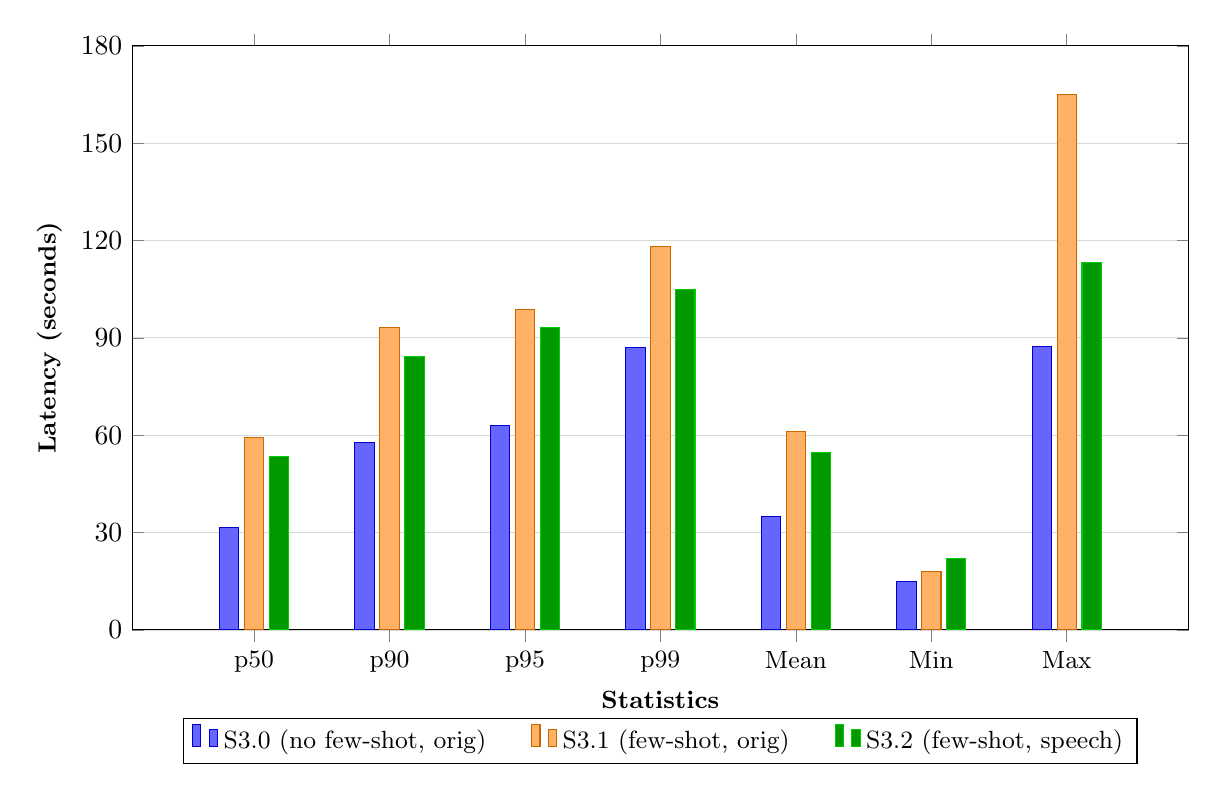
\begin{tikzpicture}
  \begin{axis}[
    width=15cm,
    height=9cm,
    ybar,
    bar width=7pt,
    ylabel={Latency (seconds)},
    ylabel style={font=\small\bfseries},
    xlabel={Statistics},
    xlabel style={font=\small\bfseries},
    symbolic x coords={p50, p90, p95, p99, Mean, Min, Max},
    xtick=data,
    xticklabel style={font=\small},
    ymin=0,
    ymax=180,
    ytick={0, 30, 60, 90, 120, 150, 180},
    ymajorgrids=true,
    grid style={line width=0.3pt, draw=gray!30},
    legend style={
      at={(0.5,-0.15)},
      anchor=north,
      legend columns=3,
      font=\small,
      /tikz/every even column/.append style={column sep=0.5cm}
    },
    enlarge x limits=0.15,
  ]
  
  % S3.0 (no few-shot, orig) - Blue
  \addplot[fill=blue!60, draw=blue!80!black] coordinates {
    (p50, 31.47)
    (p90, 57.79)
    (p95, 63.02)
    (p99, 87.16)
    (Mean, 34.83)
    (Min, 14.85)
    (Max, 87.24)
  };
  \addlegendentry{S3.0 (no few-shot, orig)}
  
  % S3.1 (few-shot, orig) - Orange
  \addplot[fill=orange!60, draw=orange!80!black] coordinates {
    (p50, 59.39)
    (p90, 93.15)
    (p95, 98.77)
    (p99, 118.28)
    (Mean, 61.09)
    (Min, 18.13)
    (Max, 164.96)
  };
  \addlegendentry{S3.1 (few-shot, orig)}
  
  % S3.2 (few-shot, speech) - Green
  \addplot[fill=green!60!black, draw=green!80!black] coordinates {
    (p50, 53.45)
    (p90, 84.15)
    (p95, 93.31)
    (p99, 104.99)
    (Mean, 54.55)
    (Min, 22.01)
    (Max, 113.26)
  };
  \addlegendentry{S3.2 (few-shot, speech)}
  
  \end{axis}
\end{tikzpicture}
\caption{Latency statistics for S3 variants (seconds).}
\label{fig:s3-latency-bar}
\end{figure}


\subsection*{Cost Analysis (S3: Multi-LLM Consensus, Full Input)}

\textbf{Assumptions.} Two parallel extractions are run on the full input: one with \textit{GPT-5} and one with \textit{Gemini~2.5~Pro}, each using $I{=}3{,}000$ input tokens and $O{=}300$ output tokens. A single arbiter/verification step runs on \textit{GPT-5-mini} with $V_{\text{in}}{=}1{,}000$ and $V_{\text{out}}{=}100$. If audio is used, Whisper transcription for $D$ minutes is added once per record.

\textbf{Prices.} GPT-5: input \$1.25/M, output \$10.00/M; GPT-5-mini: input \$0.25/M, output \$2.00/M; Gemini~2.5~Pro (prompts $\le$200k): input \$1.25/M, output \$10.00/M; Whisper: \$0.006/min.

\textbf{Formula.}
\[
\text{Cost}_{\text{S3}} =
\Big(\tfrac{I}{10^6}p_{\text{in}}^{(5)}+\tfrac{O}{10^6}p_{\text{out}}^{(5)}\Big)
+\Big(\tfrac{I}{10^6}p_{\text{in}}^{(\text{Gemini})}+\tfrac{O}{10^6}p_{\text{out}}^{(\text{Gemini})}\Big)
+\Big(\tfrac{V_{\text{in}}}{10^6}p_{\text{in}}^{(\text{mini})}+\tfrac{V_{\text{out}}}{10^6}p_{\text{out}}^{(\text{mini})}\Big)
+0.006\cdot D
\]

\textbf{Per-record (no audio).}
\[
\begin{aligned}
\text{GPT-5 extract: } & \tfrac{3000}{10^6}\!\cdot\!1.25 + \tfrac{300}{10^6}\!\cdot\!10.00 = \mathbf{\$0.00675} \\
\text{Gemini~2.5~Pro extract: } & \tfrac{3000}{10^6}\!\cdot\!1.25 + \tfrac{300}{10^6}\!\cdot\!10.00 = \mathbf{\$0.00675} \\
\text{mini arbiter: } & \tfrac{1000}{10^6}\!\cdot\!0.25 + \tfrac{100}{10^6}\!\cdot\!2.00 = \mathbf{\$0.00045} \\
\textbf{Total: } & \mathbf{\$0.01395}\ (\approx 1.40\text{¢/doc})
\end{aligned}
\]

\textbf{With audio (Whisper).} Adding Whisper introduces a linear term $0.006\cdot D$. For $D{=}1$\,min, the total cost becomes $\$0.01395 + 0.006 = \mathbf{\$0.01995}$ (approximately $2.00$\,¢ per document). Under these settings, S3 costs roughly $1.9\times$ as much as S1 (\$0.01395 vs.\ \$0.00720 per document, no audio), reflecting the dual full-input passes while keeping the arbiter overhead small compared to the extraction steps.

\subsection*{Consistency (Formatting \& Style)}

\begin{figure}[H]
\centering
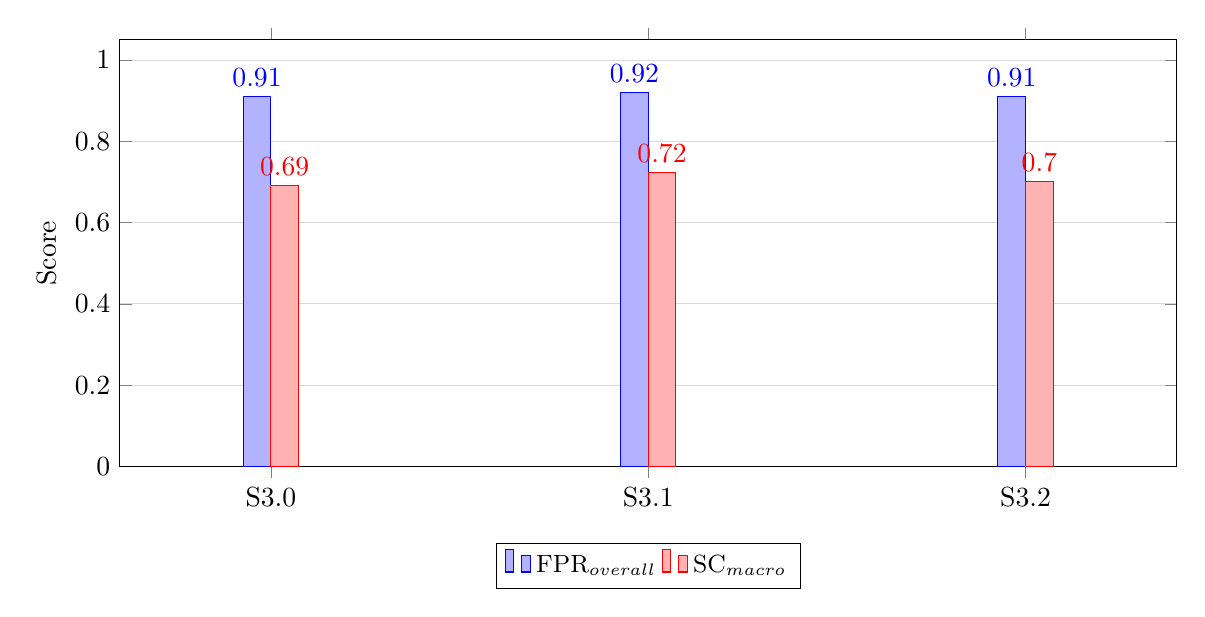
\begin{tikzpicture}
  \begin{axis}[
    width=15cm,
    height=7cm,
    ybar=0pt,
    bar width=10pt,
    ymin=0, ymax=1.05,
    ylabel={Score},
    symbolic x coords={S3.0,S3.1,S3.2},
    xtick=data,
    ymajorgrids=true,
    grid style={line width=0.3pt, draw=gray!30},
    legend style={at={(0.5,-0.18)}, anchor=north, legend columns=2, font=\small},
    enlarge x limits=0.20,
    nodes near coords,
    nodes near coords align={vertical},
  ]
    % FPR_overall
    \addplot coordinates {(S3.0,0.910) (S3.1,0.920) (S3.2,0.910)};
    \addlegendentry{$\mathrm{FPR}_{\text{overall}}$}

    % SC_macro
    \addplot coordinates {(S3.0,0.691) (S3.1,0.724) (S3.2,0.702)};
    \addlegendentry{$\mathrm{SC}_{\text{macro}}$}
  \end{axis}
\end{tikzpicture}
\caption{Consistency (S3 variants): schema formatting vs.\ input-aware style.}
\label{fig:s3-consistency}
\end{figure}

Figure~\ref{fig:s3-consistency} indicates that multi-LLM consensus maintains high structural and stylistic consistency. All S3 variants achieve $\mathrm{FPR}_{\text{overall}}{=}0.910$ or higher, with S3.1 slightly ahead at $0.920$, which shows that most outputs adhere to the expected JSON schema even after aggregation. The style-aware score $\mathrm{SC}_{\text{macro}}$ improves from $0.691$ in S3.0 to $0.724$ in S3.1, suggesting that the combination of few-shot prompting and consensus helps the system converge on more uniform phrasing and formatting across documents. S3.2, evaluated on speech-style input, remains close to S3.1 in both metrics, which indicates that the ensemble design is robust to noisier transcripts: consensus can smooth out some of the variability introduced by speech-like text while preserving schema fidelity.

Taken together, the S3 family demonstrates how full-document multi-LLM consensus trades additional cost and latency for improved calibration and robustness. Relative to the iterative S2.1 configuration, S3.1 reduces hallucinations (HR $0.301 \rightarrow 0.208$) and raises FDA (from $0.718$ to $0.743$) while also achieving higher OBS, suggesting that cross-model agreement provides more trustworthy fills at the expense of a small increase in misses. Compared to the best single-pass configuration S1.1, S3.1 reaches very similar headline scores but offers better performance on gold-nonempty slots (higher NES) and slightly lower MR, indicating stronger content quality when fields are present. The speech-style variant S3.2 maintains this pattern, trading a small decrease in overall accuracy for higher NES and stable RFA, which makes it attractive for spoken-text deployments where correctness on filled slots is more important than exploiting empty–empty alignment. Overall, S3 is best suited for settings where accuracy, calibration, and robustness justify a roughly twofold increase in LLM cost over S1 and a moderate latency premium.
